\documentclass{article}
\usepackage[utf8]{inputenc}
\usepackage{amsmath}
\usepackage{amssymb}
\usepackage{graphicx}
\usepackage{hyperref}
\usepackage{tikz}
\usepackage{pgfplots}
\usepackage{float}
\usepackage{listings}
\usepackage{color}
\usepackage{bbm}
\usepackage{multirow}

\title{Reinforcement Learning \\ Exercise 6 - Solution}
\author{Jonathan Schnitzler - st166934 \\
Eric Choquet - st160996}
\date{\today}
\begin{document}
\maketitle

\section{Planning and Learning}

\paragraph*{a) Why did Dyna-Q+ perform better in both test phase}

Lets start with the \textbf{second phase}. For the phase of the suddenly appearing shortcut in the beginning of the wall, Dyna-Q+ is able to exploit the gained benefit faster, since it generates a higher reward since the state was not visited for a long time. On the other hand Dyna-Q remains on its fixed strategy which proofed to perform better for a longer period of time(i.e. the hole on the left of the wall) and therefore remains slow. \\

Lets consider the \textbf{first phase} and the tricky question: Why doesn't it cost Dyna-Q+ to explore its environment? This can be explained by living in a grid universe and one can not exploit walking diagonal. Therefore, each path to the hole in the wall is of the same length. Dyna-Q+ performs initially better, since it tends to explore the terrain and finds the hole in the wall earlier.


\paragraph*{b) Tabular Dyna-Q algorithm}

Adaptations in order to include stochastic environments could be achieved by implementing a stochastic process in the model itself. This can be done in multiple ways, I will present two approaches here. Either, probability is directly sampled by occurence
\begin{align}
    Model(S,A) &\leftarrow R_i, S'_i \quad \text{for} i = 1,...,N \\
    Model(S, A) &:= \begin{cases} R_1, \quad x < p_1 \\
                                  \qquad \vdots \\
                                  R_j, \quad x < \sum_{i=1}^j p_j \\
                                  \qquad \vdots \\
                                  R_n, \quad x < 1
                    \end{cases}
\end{align}
where $p_j = \frac{\# R_j}{N}$ and $x$ is a random number drawn from a uniform distribution over the interval $[0, 1]$. Alternatively one can use a Kernel-interpolation, e.g. with a gaussian Kernel from each Reward (and State if they are also continuos otherwise either do first method or floor to integer representation). 

Does this still perform well on changing environments? - If not how could it? The problem is that in the planning phase the $Q$ value for the cost of the state action, could be reduced to such an extend, that it doesn't visit the state again. This can again be solved by using a term in the reward to make state which haven't benn visited for a long time more attractive via Dyna-Q+.



\section{Monte Carlo Tree Search on the Taxi environment}

\begin{figure}[H]
\centering
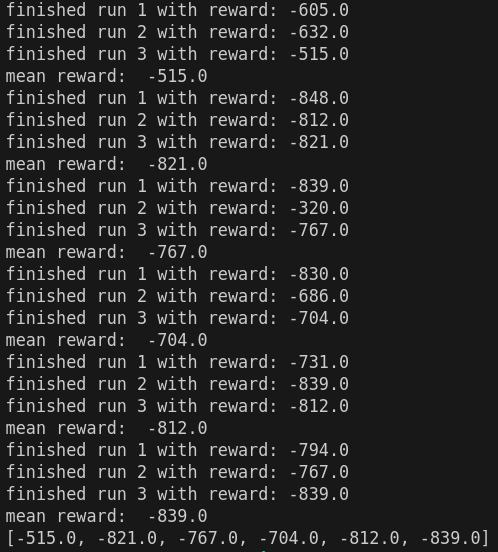
\includegraphics[width=0.5\textwidth]{images/terminal.png}
\caption{Output for Trees with \texttt{maxiter} = [10, 20, 50, 100, 200, 500]}
\label{fig:terminal}
\end{figure}
TODO:

\end{document}













